% Document For Use With LuaLaTeX
\documentclass[ngerman,a4paper,11pt]{article}

% Encoding
\usepackage[ngerman]{babel}
\usepackage{fontspec,microtype}

% Enhancements
\usepackage[all]{nowidow}
\usepackage{parskip,csquotes,xcolor}
\usepackage[labelfont=bf]{caption}

\usepackage[allpages]{continue}
\renewcommand*{\flagcont}{\bf Nächste Seite beachten! $\rightarrow$}
\renewcommand*{\flagend}{}

% Math and Science
\usepackage[locale=DE,per-mode=fraction,separate-uncertainty,sticky-per]{siunitx}
\usepackage[tbtags]{mathtools}
\usepackage{amsfonts,amssymb,physics,interval}

% Hyperref
\usepackage[colorlinks,linkcolor={red!50!black},citecolor={blue!50!black},urlcolor={blue!80!black}]{hyperref}

% Load After Hyperref
\usepackage[margin=1in,includefoot]{geometry}
\usepackage[nameinlink,noabbrev]{cleveref}
\usepackage{float,xurl}

\title{\bf Themenkreis 7: Pohlsches Rad}
\author{\sc Hüseyin Çelik}
\date{WiSe 2022/23}

\begin{document}
\maketitle
\section*{Allgemeine Hinweise}
\begin{itemize}
  \item Die Auslenkung von Erreger und Schwinger wird mit einem Winkelgeber ausgelesen. Diese sind nicht ganz linear und müssen mit einem Polynom 6. Grades kalibriert werden;
  \item Die Resonanzfrequenz \textbf{nie} ohne Dämpfung einstellen! Bei den Pohlschen Rädern liegt ein Zettel bei, welchen Wert diese für das jeweilige Gerät annimmt;
  \item Der Maximalstrom für die Spulen beträgt \SI{2}{\ampere}. Mit den verwendeten (kleinen) Netzteilen sind aber nur \SI{1.7}{\ampere} erreichbar und es ist nicht möglich, die Spulen zu zerstören. Für den aperiodischen Grenzfall wird ein anderes Netzteil zusammen mit dem Tutor verwendet;
  \item Bei Wechsel der Erregerfrequenz den Einschwingvorgang beachten.
\end{itemize}
\section*{Software}
Die Software zur Ansteuerung des Arduinos und Messung des Erregers und Oszillators wurde in \textsc{python} neu geschrieben.

Das Programm wird über die Schreibtischverknüpfung \enquote{TK7} gestartet. Das Konsolenfenster, welches sich im Hintergrund öffnet, sollte nicht geschlossen werden, kann aber ignoriert bzw. minimiert werden. Nach dem Programmstart ist in der Benutzeroberfläche nur der \enquote{CONNECT} Knopf sowie die Dropdown-Liste für den Serial Port zu sehen. Hier sollte aus der Liste der zum Arduino zugehörige COM-Port ausgewählt werden.

Nach erfolgreicher Verbindung mit dem Arduino werden in der Benutzeroberfläche die Knöpfe \enquote{START}, \enquote{STOP} und \enquote{SAVE} sowie die Eingabe für den Dateinamen und die Erregerfrequenz freigegeben (siehe \cref{fig:gui}).

Bei dem Dateinamen sollte beachtet werden, dass es sich um einen absoluten Dateipfad handelt. Soll die Datei auf dem Schreibtisch in einem Unterordner gespeichert werden, so muss dieser zuerst angelegt, und anschließend der Dateipfad in der Benutzeroberfläche ergänzt werden. \textbf{Vorhandene Dateien werden ohne zu fragen überschrieben!}

Die Messung kann mit der aktuell eingestellten Erregerfrequenz über den \enquote{START} Knopf gestartet und den \enquote{STOP} Knopf beendet werden. Wird bei laufender Messung der \enquote{START} Knopf gedrückt, so wird die Messung zunächst beendet, und bei erneutem Drücken neu gestartet. Wird bei laufender Messung der \enquote{SAVE} Knopf gedrückt, so wird die Messung beendet und die Messung mit dem angegebenen Dateinamen abgespeichert.
\begin{figure}[H]
  \centering
  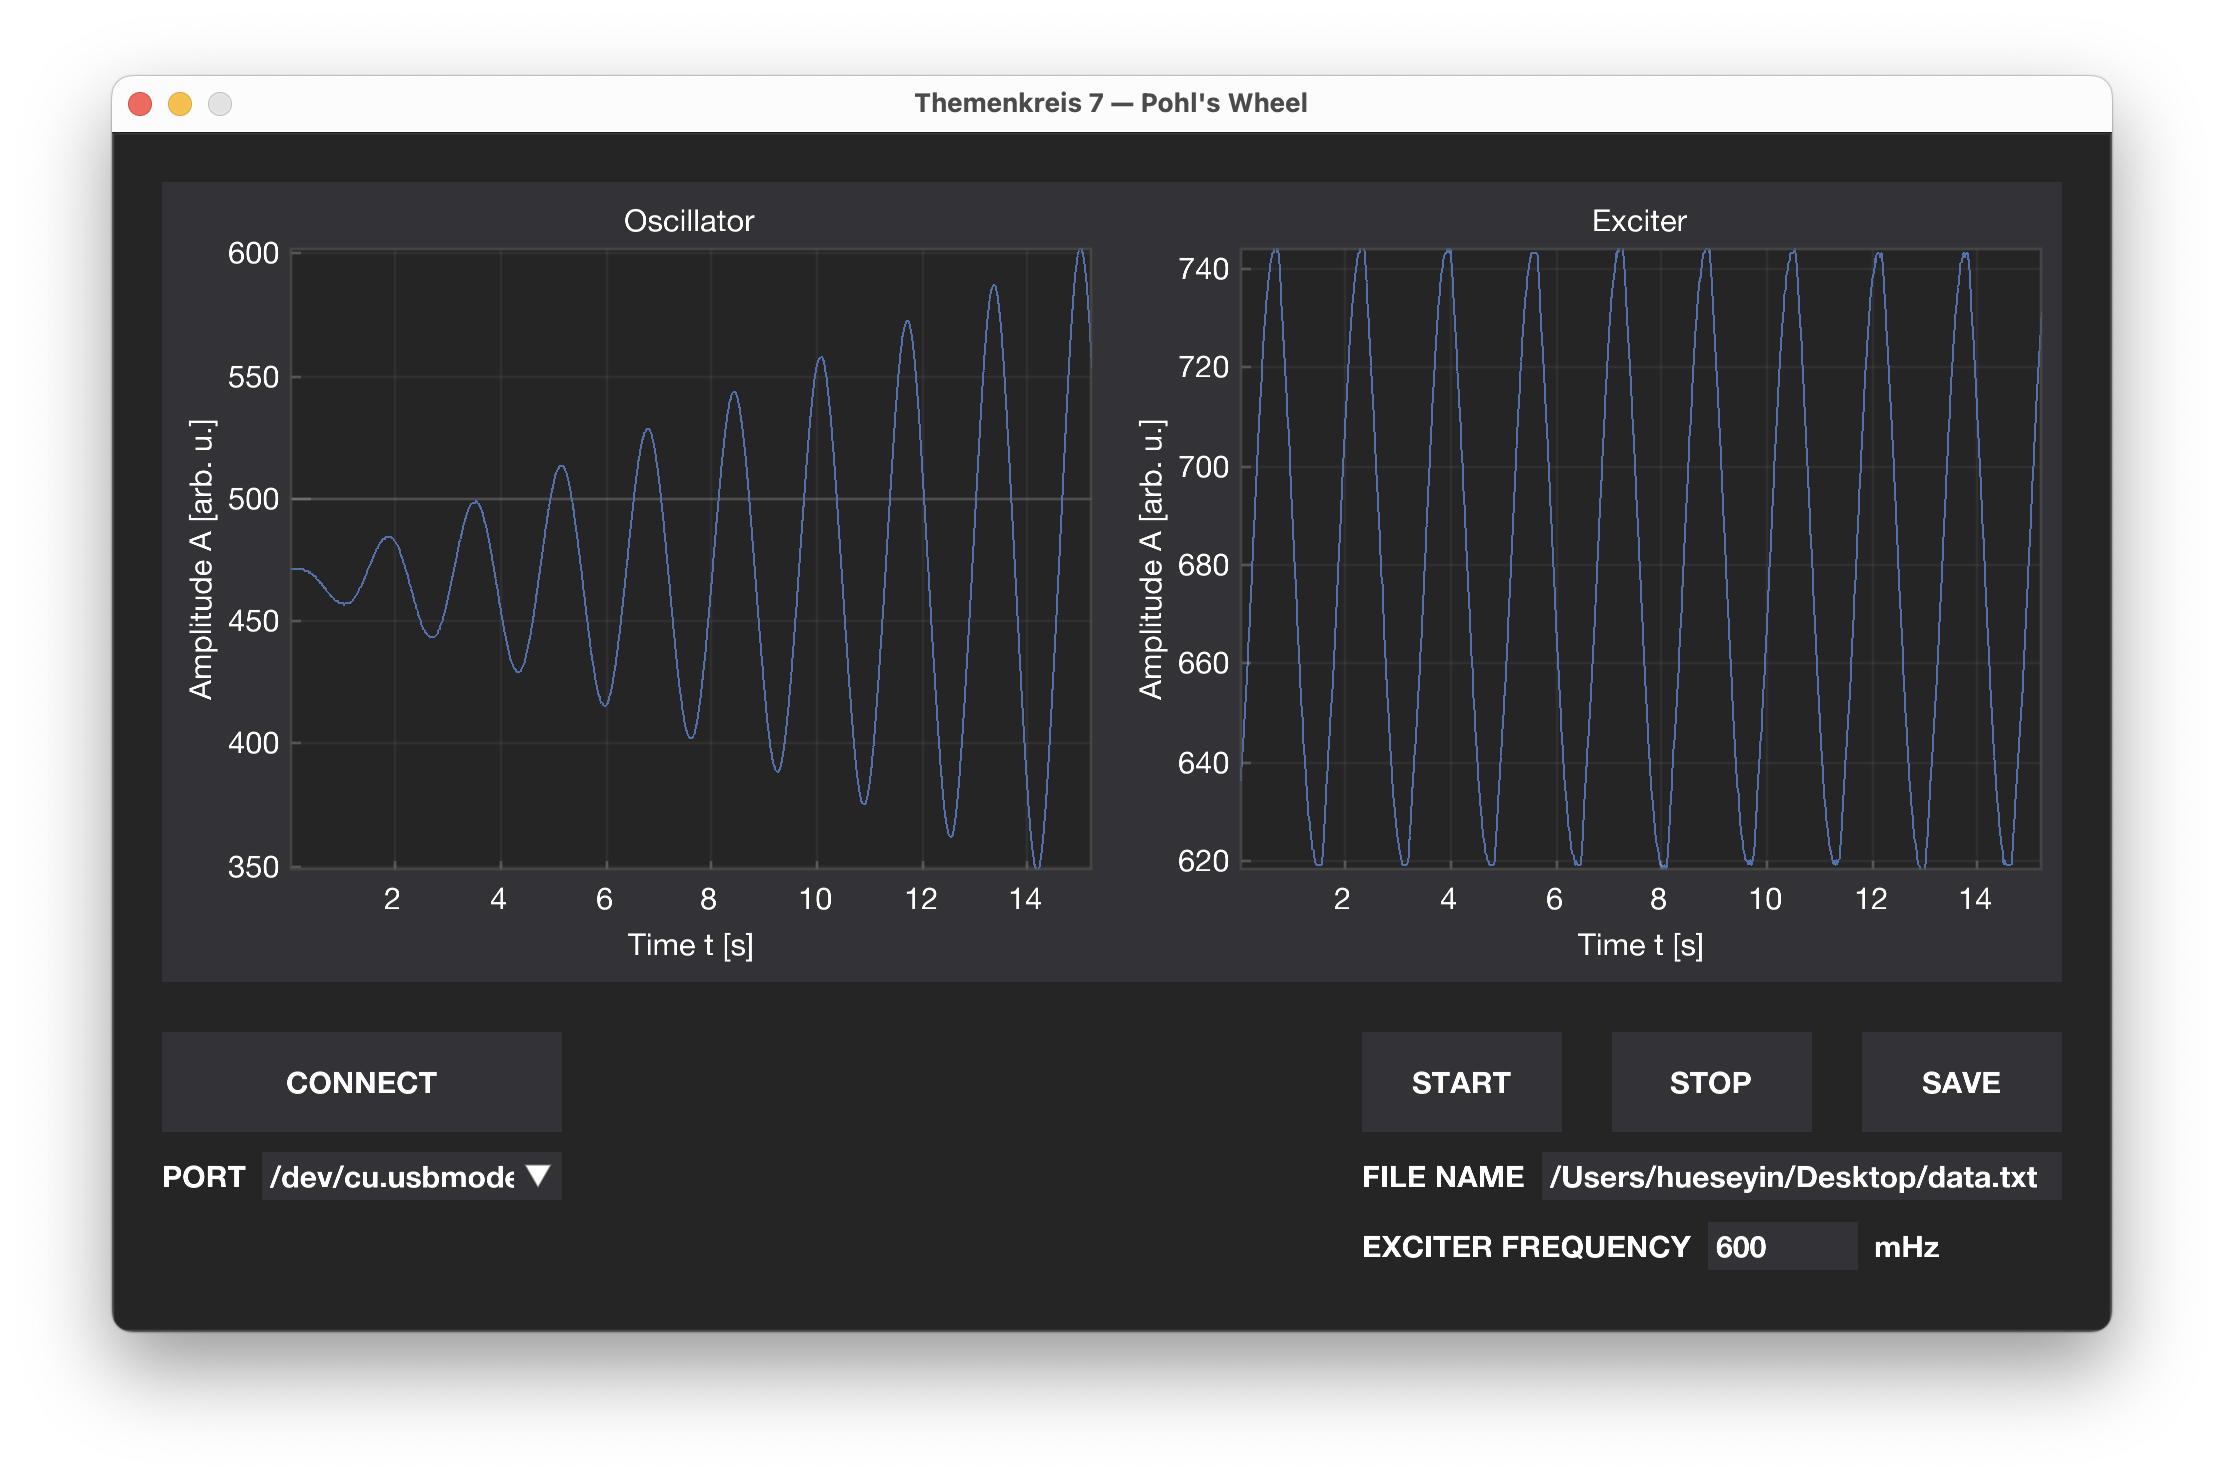
\includegraphics[width=0.8\textwidth]{screenshot-gui.png}
  \caption{GUI zur Ansteuerung des Pohlschen Rades über den Arduino sowie zur Messung der Erreger- und Oszillatorfrequenz}
  \label{fig:gui}
\end{figure}
Gelegentlich bricht die Messung nach kurzer Zeit mit der Fehlermeldung

\hspace{1em} \enquote{Error: not enough values to unpack (expected 3)! Try restarting the Arduino!}

ab. Hier muss das Programm geschlossen, und der Arduino über das Ein- und Ausstecken der Stromzufuhr neu gestartet werden.
\end{document}
